%for compilation: pdflatex psi_2015.tex 
\documentclass{llncs}

\usepackage{makeidx}  % allows for indexgeneration
\usepackage{listings}
\usepackage{algpseudocode}
\usepackage{algorithm}
\usepackage{caption}
\usepackage{algorithmicx}
%\usepackage{mathspec}
\usepackage{textcomp}
%\usepackage{subcaption}
\usepackage{graphicx}
\usepackage{epstopdf}
\usepackage{subfig} 
\sloppy

\begin{document}

\algtext*{EndWhile}% Remove "end while" text
\algtext*{EndIf}% Remove "end if" text
\algtext*{EndFor}% Remove "end for" text
\algtext*{EndFunction}% Remove "end function" text

\frontmatter          % for the preliminaries

\pagestyle{headings}  % switches on printing of running heads
\addtocmark{Hamiltonian Mechanics} % additional mark in the TOC

\title{Relaxed Parsing of Regular Approximations of String-Embedded Languages}
\titlerunning{Relaxed Parsing of Regular Approximations of String-Embedded Languages}  % abbreviated title (for running head)


\author{Ekaterina Verbitskaia\inst{1} \and Semyon Grigorev\inst{2}
\and Dmitry Avdyukhin\inst{3}}
%
%\authorrunning{Ivar Ekeland et al.} % abbreviated author list (for running head)
%

\institute{Saint Petersburg State University\\
\email{kajigor@gmail.com},
\and
\email{rsdpisuy@gmail.com}
\and
\email{dimonbv@gmail.com}}

\maketitle              % typeset the title of the contribution

\begin{abstract}
  We study conjunctive partial deduction, an advanced specialization technique aimed at improving the performance of logic programs, in the context of relational programming language \mk. We identify a number of issues, caused by  \mk pecularities, and describe a novel approach to specialization based on partial deduction and supercompilation. While the results of the evaluation do not yet demonstrate the advantages of our approach in all cases, we nevertheless consider it as the first step towards an efficient optimization framework for \mk.
\end{abstract}

\section{Introduction}

Graph querying is finding all paths in the graph which satisfy some constraints.
If the constraints are specified with some language formalism, i.e. a grammar, it is called a language-constrained path query. The simplest query described with a grammar $S \rightarrow a \ b$ being run against the graph in the Fig.~\ref{fig:exmplInputGraph} returns the only path $2, 3, 4$ (shown in red).

A grammar $S \rightarrow a \ S \ b \mid a \ b$ is a query for the paths of the form $a^n b^n$, where $n \geq 1$.
Querying the graph in the Fig.~\ref{fig:exmplInputGraph} returns the infinite set of paths one of which starts and ends in the vertex $3$ and goes around the cycles in the graph the appropriate number of times: $3,1,2,3,1,2,3,4,3,4,3,4,3$.

\begin{figure}[h]
\begin{tikzpicture}[shorten >=1pt,node distance=2cm,on grid,auto]
   \node[state] (q_1)   {$1$};
   \node[state] (q_2) [above=of q_1] {$2$};
   \node[state] (q_3) [above right=of q_1, below right=of q_2] {$3$};
   \node[state] (q_4) [right=of q_3] {$4$};
    \path[->]
    (q_1) edge  node {a} (q_2)
    (q_2) edge[red]  node {a} (q_3)
    (q_3) edge  node {a} (q_1)
    (q_3) edge[bend left, above, red]  node {b} (q_4)
    (q_4) edge[bend left, below]  node {b} (q_3);
\end{tikzpicture}
\caption{An example of input graph}
\label{fig:exmplInputGraph}
\end{figure}

Most existing graph traversing/querying languages, including SPARQL~\cite{sparql}, Cypher~\footnote{Cypher language web page: \url{https://neo4j.com/developer/cypher-query-language/}. Access date: 16.01.2018}, and Gremlin~\cite{gremlin} support only regular languages as constrains.
For some applications, regular languages are not expressive enough.
Context-free path queries (CFPQ), on which we focus this paper, employ context-free languages for constraints specification.
CFPQs are used in bioinformatics~\cite{GraphQueryWithEarley}, static code analysis~\cite{Reps, Zheng, LabelFlowCFLReachability, specificationCFLReachability, JavaCFL}, and RDF processing~\cite{CFGonRDF}.
Although there is a lot of problem-specific solutions and theoretical research on CFPQs~\cite{Yannakakis, ConjCFPathQuery, Hellings16, GrigorevR16, QueryGraphWithData, RegularDBQuery, GraphQueryWithEarley, graphDB}, cfSPARQL~\cite{CFGonRDF} is the single known graph query language to support CF constraints.
Generic solution for the integration of CFPQs into general-purpose languages is not discussed enough.

When developing a data-centric application, one wants to use a general-purpose programming language and also to have transparent and native access to data sources.
One way to achieve this is to use string-embedded DSLs.
In this approach, a query is written as a string, then passed on to a dedicated driver which executes it and returns a possibly untyped result.
Despite the simplicity, string-embedded DSLs have serious drawbacks.
First of all, they require the developer to learn the language itself, its features, runtime, and how the integration between the languages is implemented.
DSLs are also a source of possible errors and vulnerabilities, static detection of which is a serious challenge~\cite{stringEmbeddedLanguagesProblem}.
Such techniques as the Object Relationship Mapping (ORM) or Language Integrated Query~(LINQ)~\cite{LINQ1, LINQ2, LinqRDF} partially solve these problems, but they still have issues with flexibility: both query decomposition and  reusing of subqueries are a struggle.
In this paper, we propose a transparent and natural integration of CFPQs into a general-purpose programming language.

Context-free path queries are known in various domains under different names. The \emph{context-free language reachability framework} or  \emph{IFDS framework} is how they are called in the area of static code analysis.
In~\cite{Reps:1995, Reps} Thomas Reps shows that the wide range of static code analysis problems can be formulated in terms of CFL-reachability in the graph.
This framework is used for such problems as the taint analysis~\cite{CFLTaint}, the alias analysis~\cite{JavaCFL, Zheng, CFLGraspan}, the label flow analysis~\cite{LabelFlowCFLReachability}, and the fix locations problem~\cite{CFLfinding}.
What we propose in the paper can be viewed as a core of such framework since it provides both problem and domain independent mechanism for CFPQ evaluation.

We view parser combinators as the best way to integrate context-free language specifications into a general-purpose programming language. Parser combinators provide not only a transparent integration but also compile-time checks of correctness and high-level techniques for generalization. An idea to use combinators for graph traversing has already been proposed in~\cite{ScalaGraphParsing}. Unfortunately, the solution presented processes cycles in the input graph only approximately and is unable to handle left-recursive combinators, which is the most common issue of the approach. Authors pointed out that the idea described is similar to the parser combinators, but the language class supported or restrictions are not discussed.

Parser combinators are known to handle only a subset of context-free grammars: left recursion and ambiguity of the grammars are problematic.
In~\cite{Meerkat}, the authors demonstrate a set of parser combinators which handles arbitrary context-free grammars by using ideas of the Generalized LL~\cite{scott2010gll} algorithm (GLL).
Meerkat~\footnote{Meerkat project repository:~\url{https://github.com/meerkat-parser/Meerkat}. Access date: 16.01.2018} parser combinators library implements the ideas from the paper~\cite{Meerkat} and provides the parsing result in a compact form as a Shared Packed Parse Forest~\cite{SPPF}~(SPPF).
SPPF is a suitable finite structural representation of a CFPQ result, even when the set of paths is infinite~\cite{GrigorevR16}.
All the paths can be extracted from the SPPF---in the form of the corresponding derivation trees---and further analysis can be done.
It is also possible to run some further processing over the SPPF itself---not extracting the paths explicitly.

In this paper, we compose these ideas and present a set of parser combinators for context-free path querying which handles arbitrary context-free grammars and provides a structural representation of the result.
We make the following contributions in the paper.

\begin{enumerate}
\item We show that it is possible to create a set of parser combinators for context-free path querying which works on both arbitrary context-free grammars and arbitrary graphs and provides a finite structural representation of the query result.
\item We implement the parser combinators library in Scala. This library provides integration to Neo4j~\footnote{Neo4j graph database site: \url{https://neo4j.com/}. Access date: 16.01.2018} graph database. The source code is available on GitHub: \url{https://github.com/YaccConstructor/Meerkat}.
\item We perform an evaluation on realistic data and compare the performance of our library with another GLL-based CFPQ tool and with the Trails library.
We conclude that our solution is expressive and performant enough to be applied to the real-world problems.
\end{enumerate}

This paper is organized as follows.
We introduce a formal definition of the CFPQ problem in section~\ref{sec:CFPQ}, and we provide a basic description of the Meerkat library and SPPF data structure in section~\ref{sec:GLL}.
We describe our solution in section~\ref{sec:combinators}.
In section~\ref{sec:examples} we present and discuss a set of classical queries (the same generation query, the queries to a movie dataset~\footnote{The movie database is a traditional dataset for graph databases. Detailed description is available here: \url{https://neo4j.com/developer/movie-database/}. Access date: 16.01.2018})
written with our library.
Evaluation of the library is described in section~\ref{sec:evaluation}.
Finally, In section~\ref{sec:conclusion} we conclude and discuss possible directions for further research.

\section{Related Works}

Our approach for syntax analysis of string-embedded languages borrows some common principles
from existing techniques in this area. In addition, we reuse RNGLR syntax analysis algorithm 
and some accompanying constructs. In this section we provide a review and recollect some important
notions which will be referred to later on. 

\subsection{String-Embedded Languages Analysis Techniques}
The analysis of string-embedded languages, as a rule, requires a set of \emph{hotspots} to
be indicated in the host application source code. Hotspot is considered as some ``point 
of interest'', where the analysis of the set of possible string values is desirable. This task can be
performed either in a user-assisted manner or automatically using some pragmatic 
considerations or knowledge of the framework being analyzed. The following logical steps 
include static analysis to construct an approximation for the set of all possible string values,
lexical, syntax, and, perhaps, some kind of semantic analysis. These steps are not
necessarily performed separately; some of them may be omitted.

A rather natural idea of \emph{regular approximation} is to approximate the set of all possible 
strings by a regular expression. In recognition-centric formulation, this approach boils down to
the problem of inclusion of approximating regular language into context-free reference language, which
is decidable for a number of practically significant cases~\cite{LangInclusion}.
Many approaches follow this route. In~\cite{Stranger}, forward reachability analysis is used to compute regular 
approximation for all string values in the program. Further analysis is based on patterns detection in approximation 
set or generation of some finite subset of strings for analysis by standalone tools. Regular approximation in~\cite{JSA} 
is acquired by widening context-free approximation, initially built as a result of program analysis. 
Our approach is partially inspired by Alvor~\cite{Alvor,ALVOR2} which utilizes GLR-based technique for syntax 
analysis of regular approximation; this framework implements abstract lexical analysis to convert a
regular language over characters into regular language over tokens, which simplifies syntax analysis.

Kyung-Goo Doh et al. in a series of papers~\cite{AbstrParsing,LRAbstrParsing,LRAbstrParsingSema} introduced an
approach, based on implicit representation of the set of potential strings as a system of data-flow equations. 
Conventional LALR(1) is chosen for the basis of parsing algorithm; original parse tables are reused. 
Syntax analysis is performed as the system of dataflow equations is being solved iteratively in the space of abstract stacks.
The problem of infinite stack growth, which appears in general case, is handled using abstract 
interpretation~\cite{AbstractInterpretation}. This approach later evolved to a certain kind of semantic processing
in terms of attribute grammars which made it possible to analyze a wider class of languages, than
LALR(1).

\subsection{Right-Nulled Generalized LR Parsing Algorithm}
RNGLR (Right-Nulled Generalized LR) is a modification of Generalized LR (GLR) algorithm, which
was developed by Masaru Tomita~\cite{Tomita} in the context of natural language processing. 
GLR was designed to handle ambiguous context-free grammars. Ambiguities in the grammar produce 
shift/reduce and reduce/reduce conflicts, speaking in terms of LR approach. The algorithm 
uses parse tables, similar to those for classical LR, each cell of which can contain multiple 
actions. The general approach is to carry out all possible actions during parsing 
using graph-based data structures to efficiently represent the set of stacks 
and derivation trees. Originally, Tomita's algorithm was unable to recognize all context-free languages.  
Elizabeth Scott and Adrian Johnstone presented RNGLR~\cite{RNGLR},
which extends GLR with a certain way of handling \emph{right nullable} 
rules (i.e. rules of the form $\mathrm{A} \rightarrow \alpha \beta$, where $\beta$ 
reduces to an empty string).

To efficiently represent the set of all stacks produced during parsing,
RNGLR uses Graph Structured Stack (GSS). GSS is a directed graph,
whose vertices correspond to the elements of individual stacks and edges link successive
stack elements. Each vertex can have multiple incoming and outgoing edges to merge 
multiple stacks together; thus stack element sharing is implemented. Each vertex is 
a pair $(s,l)$, where $s$ is a parser state and $l$ is a \emph{level} (position in the input string). 
Vertices in GSS are unique and there are no multi-edges. 

According to RNGLR, an input is read left-to-right, one token at a time, and 
the levels of GSS are constructed sequentially for each input position: first, all  
possible reductions are applied, then the next input terminal is shifted and
pushed to the GSS. When a reduction or pushing is performed, 
the algorithm modifies GSS in the following manner. Suppose an 
edge $(v_t,v_h)$ has to be added to the GSS. By construction, the head vertex
$v_h$ is always already in the GSS. If the tail vertex is also in the GSS, then
a new edge $(v_t,v_h)$ is added (provided it is not yet there); otherwise both 
new tail vertex and new edge are created and added to the GSS. Every time a new 
vertex $v=(s,l)$ is created, the algorithm calculates the new parser 
state $s'$ from $s$ and the next terminal of the input. The pair $(v,s')$, called 
\emph{push}, is added to the global collection $\mathcal{Q}$. The set of $\epsilon$-reductions (i.e. reductions with length $l=0$) 
is also calculated, when a new vertex is added to the GSS, and reductions from this set are added to the 
global queue $\mathcal{R}$. Reductions with length $l>0$ are calculated and added to $\mathcal{R}$ 
each time a new (non-$\epsilon$) edge is created. 

An input string can have several derivation trees and, as a rule, they can have 
numerous identical subtrees. Shared Packed Parse Forest (SPPF)~\cite{SPPF} is a directed graph
designed for a compact representation of all possible derivation trees.  
SPPF has the following structure: the \emph{root} (i.e. vertex with no incoming edges) corresponds 
to the starting nonterminal of the grammar; vertices with no outgoing edges correspond to terminals 
or derivation of $\epsilon$-string; the rest of the vertices is divided into two classes: \emph{nonterminal} 
and \emph{production}. Each nonterminal vertex keeps a collection of production nodes, each of which represents one  
possible derivation of that nonterminal. Production vertices represent a right-hand side of the 
production and keep an ordered list of terminal or nonterminal nodes. The length of this list lies
in the range $[l-k..l]$, where $l$ is the length of production right-hand side, and $k$ is 
the number of rightmost symbols which derive $\epsilon$ (nullable symbols are ignored to reduce memory consumption).

SPPF is constructed simultaneously with GSS. Each edge of the GSS is associated with either 
a terminal or nonterminal node. When a GSS edge is added with a push, 
a new terminal node is created and associated with the edge. Nonterminal nodes are associated
with edges which were added, when reductions were performed: if the edge has already been in GSS, 
a production node is added to the family of nonterminal nodes, associated with the edge. All subgraphs 
from the edges of the reduction path are added as children to the production node. After the input 
is read to the end, all vertices with accepting states are searched and nodes associated with 
outgoing edges of such vertices are merged to form the resulting SPPF. All unreachable vertices 
are deleted from the SPPF graph, which leaves only the actual derivation trees for the input.

The detailed algorithm description in the form of pseudocode can be found in Appendix~\ref{RNGLRCode}.

\clearpage
\setmonofont[Mapping=tex-text]{CMU Typewriter Text}
\section{Алгоритм ослабленного синтаксического анализа регулярной аппроксимации динамически формируемого выражения}

\subsection{Описание алгоритма}
Алгоритм принимает на вход эталонную грамматику $G$ над алфавитом терминальных символов $T$ и детерминированный конечный автомат $(Q,\Sigma,\delta,q_0,q_f)$, имеющий одно стартовое состояние $q_0$, одно конечное состояние $q_f$, без $\epsilon$-переходов, где $\Sigma \subseteq T$~--- алфавит входных символов, $Q$~--- множество состояний, $\delta$~--- отношение перехода. По описанию  грамматики генерируются управляющие RNGLR-таблицы и некоторая вспомогательная информация (называемая $parserSource$ в псевдокоде).

\begin{algorithm}[!ht]
\begin{algorithmic}[1]
\caption{Алгоритм ослабленного синтаксического анализа регулярной аппроксимации динамически формируемого выражения}
\label{parsing}
\Function{parse}{$grammar, automaton$}
  \State{$inputGraph \gets$ construct inner graph representation of $automaton$}
  \State{$parserSource \gets$ generate RNGLR parse tables for $grammar$}
  \If{$inputGraph$ contains no edges}
    \If{$parserSource$ accepts empty input} {report success}
    \Else { report failure}
    \EndIf
  \Else
    \State{\Call{addVertex}{$inputGraph.startVertex, startState$}}
    \State{$\mathcal{Q}.Enqueue(inputGraph.startVertex)$}
    \While{$Q$ is not empty}
      \State{$v \gets \mathcal{Q}.Dequeue()$}
      \State{\Call{makeReductions}{$v$}}
      \State{\Call{push}{$v$}}
      \State{\Call{applyPassingReductions}{$v$}}
    \EndWhile
    \If{$\exists v_f: v_f.level = q_f$ and $v_f.state$ is accepting} {report success}
    \Else { report failure}
    \EndIf
  \EndIf
\EndFunction
\end{algorithmic}
\end{algorithm}

Алгоритм производит обход графа входного автомата и последовательно строит GSS тем же способом, как это делает RNGLR-алгоритм. Однако, так как мы имеем дело с графом вместо линейного потока, понятие следующего символа трансформируется во \emph{множество терминальных символов}, лежащих на всех исходящих рёбрах данной вершины, что несколько изменяет операции shift и reduce (смотри строку 5 в алгоритме~\ref{processVertex} и строки 9 и 21 в алгоритме~\ref{gss_construction}). Для того, чтобы управлять порядком обработки вершин входного графа, мы используем глобальную очередь $\mathcal{Q}$. Каждый раз, когда добавляется новая вершина GSS, сначала необходимо произвести все свёртки длины 0, после чего выполнить сдвиг следующих токенов со входа. Таким образом необходимо добавить соответствующую вершину графа в очередь на обработку. Добавление нового ребра GSS может порождать новые свёртки, таким образом в очередь на обработку необходимо добавить вершину входного графа, которой соответствует начальная вершина добавленного ребра. Детальное описание процесса построения GSS приведено в алгоритме~\ref{parsing}. Свёртки производятся вдоль путей в GSS, и если было добавлено ребро, начальная вершина которого ранее присутствовала в GSS, необходимо заново вычислить проходящие через эту вершину свёртки (смотри функцию applyPassingReductions в алгоритме~\ref{processVertex}).

\begin{algorithm}[H]
\begin{algorithmic}[1]
\caption{Обработка вершины внутреннего графа}
\label{processVertex}
\Function{push}{$innerGraphV$}
  \State{$\mathcal{U} \gets$ copy $innerGraphV.unprocessed$}
  \State{clear $innerGraphV.unprocessed$}
  \ForAll{$v_{h}$ in $\mathcal{U}$}  
    \ForAll{$e$ in outgoing edges of $innerGraphV$}
      \State{$push \gets$ calculate next state by $v_{h}.state$ and the token on $e$}
      \State{\Call{addEdge}{$v_{h}, e.Head, push, false$}}
      \State{add $v_{h}$ in $innerGraphV.processed$}
    \EndFor
  \EndFor
\EndFunction

\Function{makeReductions}{$innerGraphV$}
  \While{$innerGraphV.reductions$ is not empty}
    \State{$(startV, N, l) \gets innerGraphV.reductions.Dequeue()$}
    \State{find the set of vertices $\mathcal{X}$ reachable from $startV$}
    \State{    along the path of length ($l-1$), or $0$ if $l=0$;}
    \State{add $(startV, N, l-i)$ in $v.passingReductions$,}
    \State{    where $v$ is an $i$-th vertex of the path}
    \ForAll{$v_{h}$ in $\mathcal{X}$}
      \State{$state_{t} \gets$ calculate new state by $v_{h}.state$ and nonterminal $N$}
      \State{\Call{addEdge}{$v_{h}, startV, state_{t}, (l=0)$}}
    \EndFor
  \EndWhile
\EndFunction

\Function{applyPassingReductions}{$innerGraphV$}
  \ForAll{$(v, edge)$ in $innerGraphV.passingReductionsToHandle$}
    \ForAll{$(startV, N, l) \gets v.passingReductions.Dequeue()$}
      \State{find the set of vertices $\mathcal{X}$,}
      \State{    reachable from $edge$ along the path of length ($l-1$)}
      \ForAll{$v_{h}$ in $\mathcal{X}$}
        \State{$state_{t} \gets$ calculate new state by $v_{h}.state$ and nonterminal $N$}
        \State{\Call{addEdge}{$v_{h}, startV, state_{t}, false$}}
      \EndFor
    \EndFor
  \EndFor
\EndFunction
\end{algorithmic}
\end{algorithm}

Так же как и RNGLR, мы ассоциируем вершины GSS с позициями входного графа, однако в нашем случае уровень вершины~--- это состояние входного автомата. Мы строим внутреннюю структуру данных (в дальнейшем изложении называемую \emph{внутренним графом}) посредством копирования графа входного автомата и ассоциации с его вершинами следующих коллекций.
\begin{itemize}
  \item \emph{processed}: вершины GSS, для которых ранее были вычислены все операции push. Это множество агрегирует все вершины GSS, ассоциированные с вершиной внутреннего графа.
  \item \emph{unprocessed}: вершины GSS, операции push для которых ещё только предстоит выполнить. Это множество аналогично множеству $\mathcal{Q}$ алгоритма RNGLR.
  \item \emph{reductions}: очередь, аналогичная очереди $\mathcal{R}$ RNGLR-алгоритма: все операции reduce, которые ещё только предстоит выполнить.
  \item \emph{passingReductionsToHandle}: пары из вершины GSS и ребра GSS, вдоль которых необходимо осуществлять проходящие свёртки.
\end{itemize}

\begin{algorithm}[H]
\begin{algorithmic}[1]
\caption{Построение GSS}
\label{gss_construction}
\Function{addVertex}{$innerGraphV, state$}
  \State{$v \gets$ find a vertex with state $=state$ in}
  \State{    $innerGraphV.processed \cup innerGraphV.unprocessed$}
  \If{$v$ is not $null$ } \Comment{Вершина была найдена в GSS}
    \State{\Return{($v, false$)}} 
  \Else
    \State{$v \gets$ create new vertex for $innerGraphV$ with state $state$}
    \State{add $v$ in $innerGraphV.unprocessed$}
    \ForAll{$e$ in outgoing edges of $innerGraphV$}
      \State{calculate the set of zero-reductions by $v$}
      \State{    and the token on $e$ and add them in $innerGraphV.reductions$}
    \EndFor
    \State{\Return{$(v, true$)}}
  \EndIf
\EndFunction

\Function{addEdge}{$v_{h}, innerGraphV, state_{t}, isZeroReduction$}
  \State{$(v_{t}, isNew) \gets$ \Call{addVertex}{$innerGraphV, state_{t}$}}
  \If{GSS does not contain edge from $v_{t}$ to $v_{h}$}
    \State{$edge \gets$ create new edge from $v_{t}$ to $v_{h}$}
    \State{$\mathcal{Q}.Enqueue(innerGraphV)$}
    \If{not $isNew$ and $v_{t}.passingReductions.Count>0$}
      \State{add $(v_{t}, edge)$ in $innerGraphV.passingReductionsToHandle$}
    \EndIf
    \If{not $isZeroReduction$}
      \ForAll{$e$ in outgoing edges of $innerGraphV$}
        \State{calculate the set of reductions by $v$}
        \State{    and the token on $e$ and add them in $innerGraphV.reductions$}
      \EndFor
    \EndIf
  \EndIf
\EndFunction
\end{algorithmic}
\end{algorithm}

Помимо состояния анализатора $state$ и уровня $level$ (который совпадает с состоянием входного автомата), в вершине GSS хранится коллекция \emph{проходящих свёрток}. Проходящая свёртка~--- это тройка $(startV, N, l)$, соответствующая свёртке, чей путь содержит данную вершину GSS. Аналогичная тройка используется в RNGLR-алгоритме для описания свёртки, но в данном случае $l$ обозначает длину оставшейся части пути. Проходящие свёртки сохраняются в каждой вершине пути (кроме первой и последней) во время поиска путей в функции $makeReductions$ (см. алгоритм~\ref{processVertex}).

\subsection{Построение компактного представления леса разбора}
В качестве компактного представления леса разбора всех корректных выражений из множества значений динамически формируемого выражения используется граф SPPF. Построение компактного представления осуществляется одновременно с синтаксическим разбором во время построения графа стеков GSS, также как и в алгоритме RNGLR.

С каждым ребром GSS ассоциируется список лесов разбора фрагмента выражения. В графе GSS нет кратных рёбер, поэтому если во время работы функции \emph{addEdge} в нем было найдено добавляемое ребро, то с ним ассоциируется новый лес разбора, при этом в очередь на обработку не добавляется никаких вершин входного графа.  

При добавлении в GSS ребра, соответствующего считанной со входа лексеме, создаётся (и ассоциируется с ним) граф из одной терминальной вершины. Так как входной автомат является детерминированным, с ребром GSS ассоциируется не более одного такого графа.

При обработке свёртки алгоритм осуществляет поиск всех путей в графе GSS заданной длины, после чего происходит добавление в GSS новых рёбер, соответствующих данной свёртке. С каждым таким ребром ассоциируется лес, имеющий в качестве корня (вершины, у которой нет входных рёбер) вершину, соответствующую нетерминалу, к которому осуществлялась свёртка. Ребра каждого из найденных путей, перечисленные в обратном порядке, образуют правую часть некоторого правила грамматики, по которому осуществляется свёртка. Для каждого пути создаётся вершина, помеченная номером такого правила, и добавляется в лес как непосредственно достижимая из корня. Каждое ребро пути ассоциировано со списком лесов вывода символа из правой части правила. Непосредственно достижимыми вершинами вершины-правила становятся ссылки на такие списки, за счёт чего осуществляется переиспользование фрагментов леса.

В алгоритме RNGLR наличие нескольких путей, вдоль которых осуществляется свёртка к нетерминалу, означает существование более чем одного варианта вывода нетерминала. В нашем случае данная ситуация соответствует различным фрагментам нескольких выражений из входного регулярного множества, которые сворачиваются к одному нетерминалу. 

В конце работы алгоритма осуществляется поиск рёбер GSS, для каждого из которых верно, что конечная вершина имеет уровень, равный финальному состоянию входного автомата, и принимающее состояние (accepting state). Результирующее представление леса разбора получается путём удаления недостижимых вершин из графа, созданного объединением лесов разбора, ассоциированных с найденными рёбрами GSS.

Рассмотрим следующий фрагмент кода, динамически формирующий выражение \emph{expr} в строке 4. 
\begin{verbatim}
1 string expr = "" ;
2 for(int i = 0; i < len; i++) 
3 {
4     expr = "()" + expr;
5 }
\end{verbatim}

Множество значений выражения \emph{expr} аппроксимируется регулярным выражением $(\mbox{\texttt{LBR }} \mbox{\texttt{RBR}})*$, где $\mbox{\texttt{LBR }}$ соответствует открывающейся скобке, а $\mbox{\texttt{RBR}}$~--- закрывающейся. Граф конечного автомата, задающего такую аппроксимацию, изображён на рисунке~\ref{input}.
\begin{figure}[!h]
 \centering
 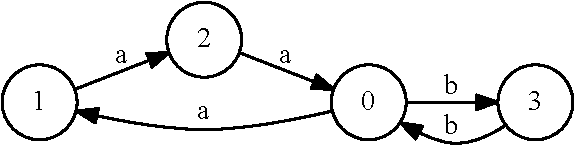
\includegraphics[]{pics/input.pdf}
 \caption{Конечный автомат, задающий регулярную аппроксимацию выражения \emph{expr}}
 \label{input}
\end{figure}

В результате работы предложенного алгоритма будет получено конечное представление леса разбора SPPF, изображённое на рисунке~\ref{sppf}.
\begin{figure}[!h]
 \centering
 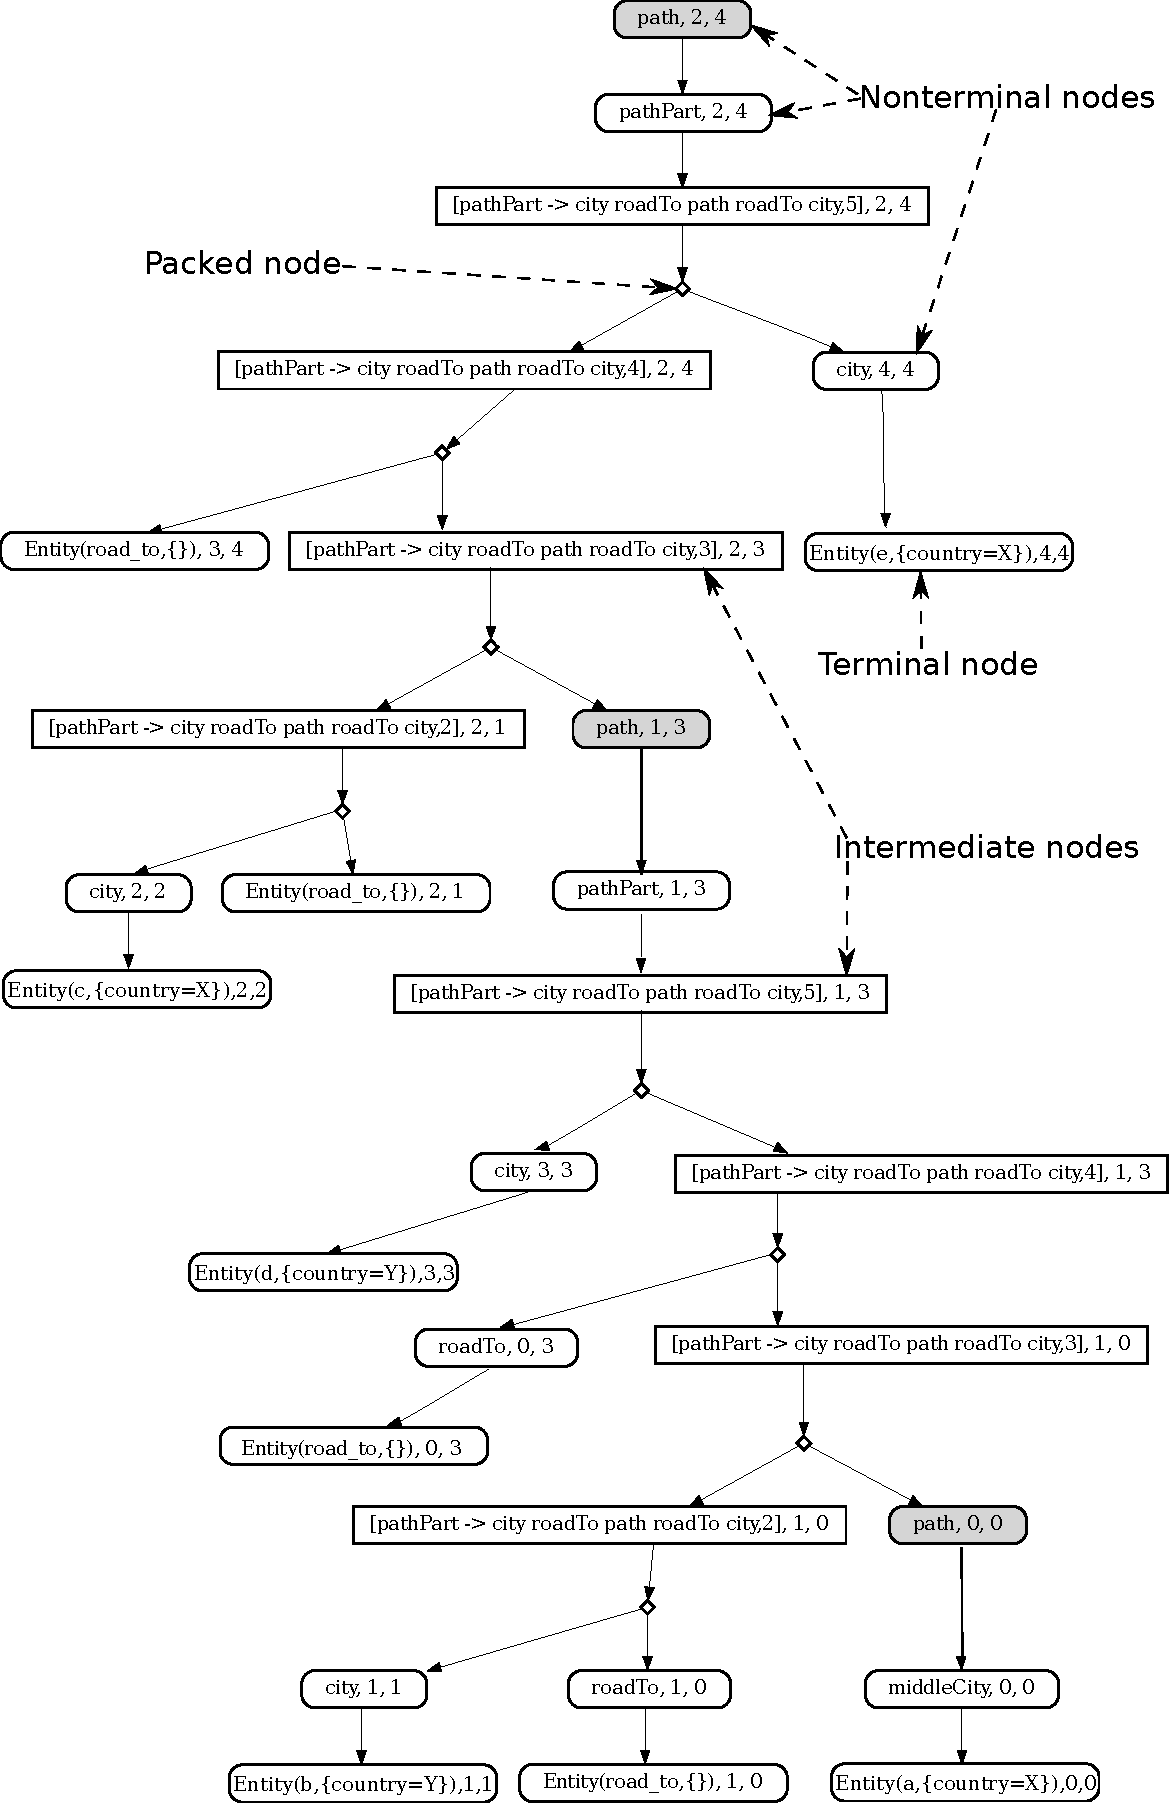
\includegraphics[width=15cm]{pics/sppf.pdf}
 \caption{Конечное представление леса разбора для выражения \emph{expr}}
 \label{sppf}
\end{figure}

%\begin{figure}[!h]
% \centering
% 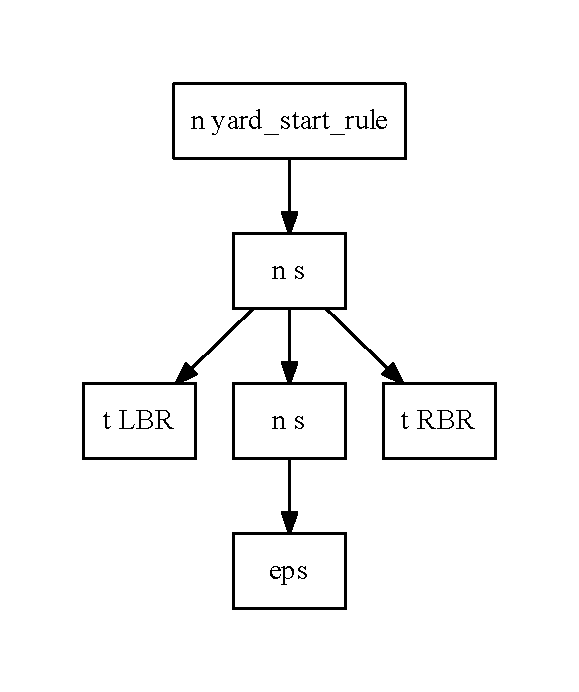
\includegraphics[]{pics/sppf1.pdf}
% \caption{Дерево вывода для выражения $expr="()"$}
% \label{sppf1}
%\end{figure}
%\begin{figure}[!h]
% \centering
% 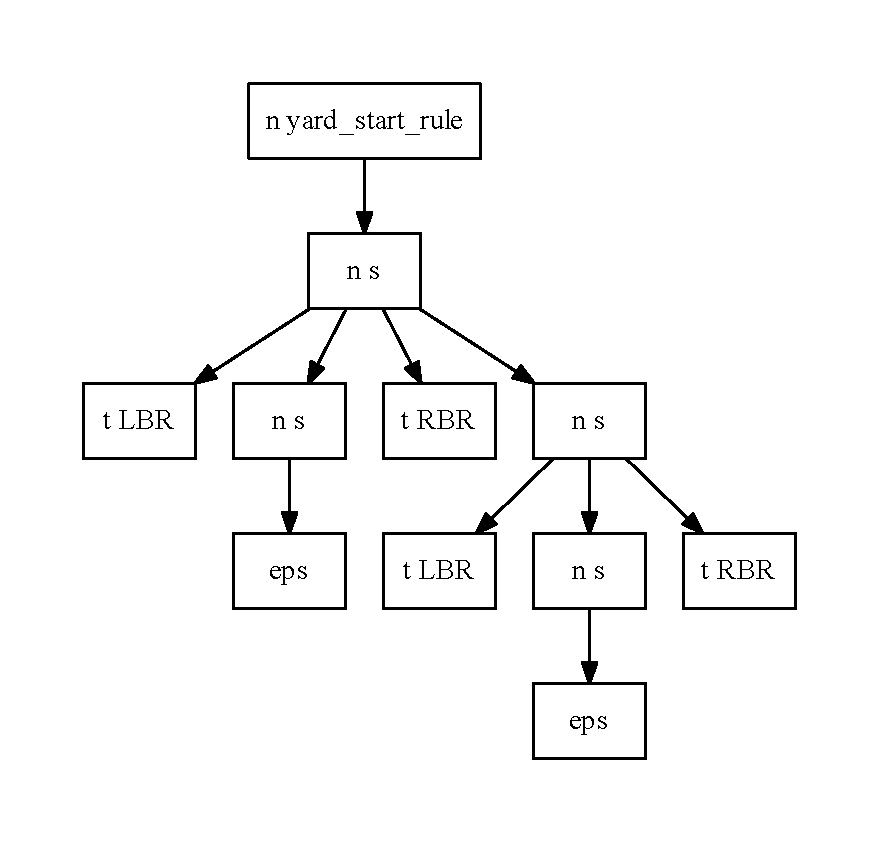
\includegraphics[]{pics/sppf2.pdf}
% \caption{Дерево вывода для выражения $expr="()()"$}
% \label{sppf2}
%\end{figure}
\begin{figure}[!h]
 \centering
 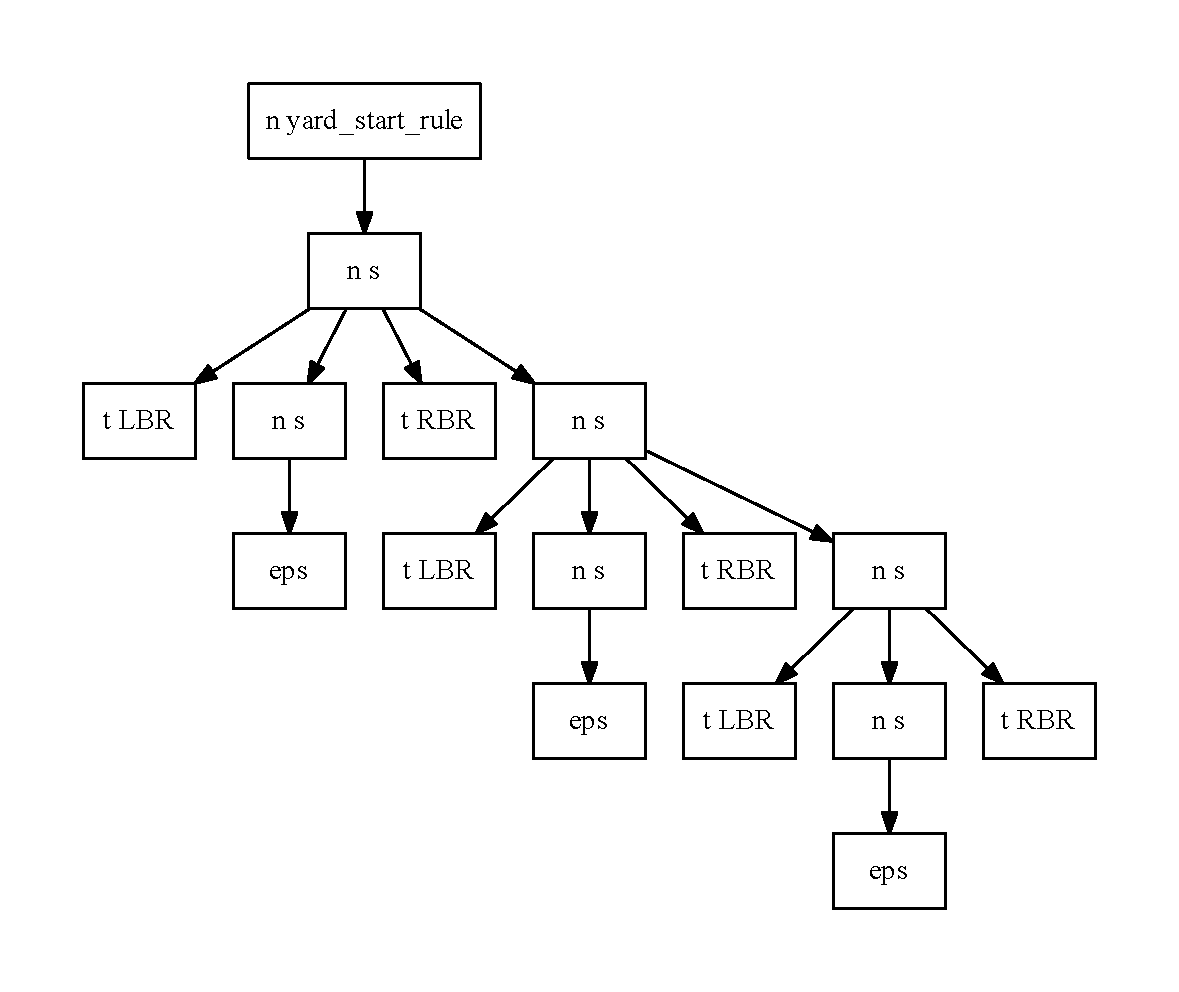
\includegraphics[width=15cm]{pics/sppf3.pdf}
 \caption{Дерево вывода для выражения $expr="()()()"$}
 \label{sppf3}
\end{figure}

Из SPPF можно извлечь бесконечное количество деревьев, каждое из которых является деревом вывода некоторого выражения из регулярной аппроксимации. Рисунок~\ref{sppf3} демонстрирует одно из таких деревьев разбора. 
%\section{Correctness of the Algorithm}
In this section we prove the correctness of the algorithm proposed, namely \textsc{Theorem 1} proves its termination,
and \textsc{Theorem 2} and \textsc{Theorem 3} prove correctness of parse forest construction.
In \textsc{Definition}, we slightly redefine classical notion of correct parse tree to better suit our problem. 
SPPF construction is inherited from RNGLR-algorithm, so the proofs are presented
in terms of GSS construction correctness. 

\textsc{Theorem 1.}
\textit{Algorithm terminates for any input.}

\textsc{Proof.}
Each vertex of inner representation of the input finite automaton contains, at most, 
$N$ GSS vertices, where $N$ is a number of parser states. So, the total number of 
GSS vertices is, at most, $N\times n$, where $n$ is the number of vertices in the inner graph. 
Since GSS has no multi-edges, the number of its edges is $O((N\times n)^2)$. The algorithm 
dequeues vertex to be processed from $\mathcal Q$ in the each iteration of the 
main loop. Vertices are enqueued to $\mathcal Q$ only when a new edge is added to GSS. Since the number of 
GSS edges is finite, the algorithm always terminates. \qed

\textsc{Definition.} 
\emph{Correct tree} is an ordered tree with the following properties:
\begin{enumerate}
  \item The root is the start nonterminal of the grammar $G$.
  \item The leaf nodes are terminals of $G$. The sequence of the leaf nodes 
        corresponds to some path in the inner graph. 
  \item The interior nodes are nonterminals of $G$. All children of nonterminal 
        $N$ correspond to the symbols of the right-hand side of some production for $N$ in $G$.
\end{enumerate}

\textsc{Lemma.}
For every GSS edge $(v_{t}, v_{h})$, $v_{t} \in V_{t}.processed$, $v_{h} \in V_{h}.processed$, 
the terminals of the associated subtree correspond to some path in the inner graph $p$ 
from $V_{h}$ to $V_{t}$.

\textsc{Proof.}
The proof is by induction on the height of derivation tree. 
The base case is either some $\epsilon$-tree or a tree with the single leaf. An $\epsilon$-tree corresponds 
to a path of zero length; the tail and the head of the edge associated with $\epsilon$-tree are identical, 
thus the statement is true. A tree with the single leaf corresponds to a single terminal read from an edge 
($V_{h}$, $V_{t}$) of the inner graph, thus the statement is true.

A tree of height $k$ has a nonterminal $N$ as its root. By third statement of correct tree definition, 
there is a production $N \rightarrow A_{0}, A_{1}, \dots, A_{n}$ for children $A_{0}, A_{1}, \dots, A_{n}$ of the root node. 
A subtree $A_{i}$ is associated with GSS edge $(v_{t}^{i}, v_{h}^{i})$ and, as its height is $k-1$, by inductive hypothesis,
there is a path in the inner graph from $V_{h}^{i}$ to $V_{t}^{i}$. $V_{t}^i = V_{h}^{i+1}$, since $v_{t}^i = v_{h}^{i+1}$, 
thus there is a path in the inner graph from $V_{h}^{0}$ to $V_{t}^{n}$, corresponding to the tree under consideration.
\qed

\textsc{Theorem 2.} 
\textit{Every generated from SPPF tree is correct.}

\textsc{Proof.} Consider arbitrary tree, generated from SPPF, and prove that it is correct. The first and the third statements
of correctness definition immediately follow from SPPF definition. 

{\bf (did'not understand the following statement; Russian decryption is required:)}
\textsc{Lemma 1} proves the second item of the definition by consideration of all the edges from the GSS vertex
on the last level having accepting state to the vertex on the 0-level with the start parser state.

\qed

\textsc{Theorem 3.} 
\textit{For every path $p$ in the inner graph, a correct tree corresponding to $p$ can be generated from SPPF.}

\textsc{Proof.}
Consider arbitrary correct tree and show it can be generated from SPPF. The proof follows the proof of correctness 
for RNGLR-algorithm, except the following moment. RNGLR constructs GSS layer-by-layer: it is guaranteed, that $j$-th 
level of the GSS $\forall j \in [0..i-1]$ would be fixed by the time, when $i$-th level is processed. In our case, 
this property does not hold, which leads to possible generation of the paths for reductions already applied. 
The only possible way to actually add a new path is to add an edge $(v_{t}, v_{h})$, where $v_{t}$ is already in the GSS and 
it has incoming edges. Since the algorithm stores, which reductions have passed through each vertex, it is sufficient to 
{\bf (what does it mean: ``continue passing reductions?'')} continue passing reductions, stored in $v_{t}$ to overcome this problem, 
and this is exactly what \emph{applyPassingReductions} function does. 
\qed

% У заключения нет номера главы
\clearpage

\section*{Заключение}
В ходе данной работы получены следующие результаты. 
\begin{itemize}
  \item Изучена предметная область: методы обработки встроенных языков и алгоритм обобщённого синтаксического анализа RNGLR.
  \item Разработан алгоритм синтаксического анализа динамически формируемых выражений, поддерживающий работу с произвольными входными графами.
  \item Доказана корректность алгоритма:
  \begin{itemize}
    \item алгоритм завершит работу для любых входных данных;
          %для любой входной детерминированной контекстно-свободной грамматики и 
          %произвольного входного графа алгоритм завершит свою работу;
    \item для любой цепочки из входного множества, выводимой в эталонной грамматике G, в SPPF содержится её дерево вывода в G; при этом никакие другие деревья не содержатся в SPPF.
          %для любой цепочки, которую может породить автомат (которая содержится 
          %в регулярном множестве), выводимой в рассматриваемой грамматике G, в 
          %SPPF содержится её дерево вывода в G, при этом не содержится никаких 
          %других деревьев.
  \end{itemize}
  \item Выполнена реализация алгоритма на языке программирования F\# в рамках исследовательского проекта YaccConstructor.
  \item Проведена апробация: регрессионное тестирование, тестирование производительности и тестирование на реальных данных.
  \item Исходный код проекта YaccConstructor можно найти на сайте \url{https://github.com/YaccConstructor/YaccConstructor}, автор принимал участие под учётной записью kajigor.
\end{itemize}

В дальнейшем планируется изменить алгоритм таким образом, чтобы помимо 
построения леса разбора всех корректных выражений осуществлялся бы также поиск ошибочных выражений и сообщение о них. Также необходимо произвести теоретическую оценку сложности алгоритма. Предложенный алгоритм планируется внедрить в инструмент по реинжинирингу информационных систем.  

%
% ---- Bibliography ----
%
\begin{thebibliography}{}
%
\bibitem{DSQLISO}
ISO. ISO/IEC 9075:1992. Information Technology~--- Database Languages~--- SQL, 1992.

\bibitem{JSP}
Damon Houglan, Aaron Tavistock. Core JSP // Prentice Hall PTR, Upper Saddle River, NJ, USA, 2000, 416~p.

\bibitem{RNGLR}
Elizabeth Scott, Adrian Johnstone.
Right Nulled GLR Parsers // ACM Trans. Program. Lang. Syst., Vol.~28, \textnumero~4,
2006, P.~577--618.

\bibitem{SPPF}
Jan Rekers.
Parser Generation for Interactive Environments. PhD Thesis. University of Amsterdam, 1992, 174~p.

\bibitem{LangInclusion}
Peter R. J. Asveld, Anton Nijholt.
The Inclusion Problem for Some Subclasses of Context-free Languages //
Theoretical Computer Science, Vol.~230, \textnumero~1-2, 1999, P.~247--256.

\bibitem{Stranger}
Fang Yu, Muath Alkhalaf, Tevfik Bultan, Oscar H. Ibarra.
Automata-based Symbolic String Analysis for Vulnerability Detection //
Formal Methods in System Design, Vol.~44, \textnumero~1, 2014, P.~44--70.

\bibitem{JSA}
Aske Simon Christensen, Anders M{\o}ller, Michael I. Schwartzbach.
Precise Analysis of String Expressions //
Proceedings of the 10th International Conference on Static Analysis, 2003, P.~1--18.

\bibitem{Alvor}
Aivar Annamaa, Andrey Breslav, Jevgeni Kabanov, Varmo Vene.
An Interactive Tool for Analyzing Embedded SQL Queries //
Proceedings of the 8th Asian Conference on Programming Languages and Systems, 2010, P.~131--138.

\bibitem{ALVOR2}
Aivar Annamaa, Andrey Breslav, Varmo Vene. Using Abstract Lexical Analysis and Parsing to Detect 
Errors in String-Embedded DSL Statements // 
Proceedings of the 22nd Nordic Workshop on Programming Theory, 2010, P.~20--22. 

\bibitem{AbstrParsing}
Kyung-Goo Doh, Hyunha Kim, David A. Schmidt. Abstract Parsing: Static Analysis of 
Dynamically Generated String Output Using LR-parsing Technology // 
Proceedings of the 16th International Symposium on Static Analysis, 2009, P.~256--272.

\bibitem{LRAbstrParsing}
Kyung-Goo Doh, Hyunha Kim, David A. Schmidt. Abstract LR-parsing // Formal Modeling, 2011, P.~90--109.

\bibitem{LRAbstrParsingSema}
Kyung-Goo Doh, Hyunha Kim, David A. Schmidt. Static Validation of Dynamically Generated HTML 
Documents Based on Abstract Parsing and Semantic Processing // 
Proceedings of the 20th International Symposium on Static Analysis, 2013, P.~194--214.

\bibitem{AbstractInterpretation} 
Patrick Cousot, Radhia Cousot. Abstract Interpretation: a Unified Lattice Model for Static Analysis 
of Programs by Construction or Approximation of Fixpoints // Proceedings of the 4th Symposium on Principles of Programming Languages, 1977, P.~238--252.

\bibitem{Tomita}
Masaru Tomita.
An Efficient All-paths Parsing Algorithm for Natural Languages //
Carnegie-Mellon University, Dept. of Computer Science, 1984.

%\bibitem{SELinIDE}
%Semen Grigorev, Ekaterina Verbitskaia, Andrey Ivanov, Marina Polubelova, Ekaterina Mavchun.
%String-embedded Language Support in Integrated Development Environment //
%Proceedings of the 10th Central and Eastern European Software Engineering Conference in Russia, 2014, P.~21:1--21:11.
%
%\bibitem{MohriNederhof}
%Mehryar Mohri, Mark-jan Nederhof.
%Regular Approximation of Context-Free Grammars Through Transformation //
%Robustness in Language and Speech Technology, Kluwer Academic Publishers, 2001, P.~153--163. 
%
%\bibitem{EvalToStaged}
%Martin Lester, Luke Ong, Max Sch{\"{a}}fer.
%Information Flow Analysis for a Dynamically Typed Language with Staged Metaprogramming //
%Proceedings of the 26th Computer Security Foundations Symposium, 2013, P.~209--223.
\end{thebibliography}

\newpage

\section*{Appendix}

We thank the reviewers for their thoughtful feedback.


\subsection*{Review 1}

The paper considers the optimisation of miniKanren relational programs using some form of (conjunctive) partial evaluation. In particular, the authors propose a novel approach, called conservative partial deduction, and reports on an experimental evaluation that compares the results obtained with ECCE (an online partial evaluator for Prolog based on conjunctive partial deduction) and the authors' tool. The results are very promising and show the advantages of the new approach.

All in all, the paper contains interesting ideas and I recommend it to be accepted for VPT 2021.

% \emph{Thank you for the kind review.}

Detailed comments for authors:

\begin{itemize}
  \item In order for the paper to be as self-complete as possible, I'd suggest to add a brief introduction to miniKanren (syntax, informal semantics, a couple of examples) at the beginning of the paper.

  \emph{Added. See subsection \ref{mkIntro}.}

  \item There are already some works that considered non-leftmost unfolding during partial evaluation, e.g.,

  \begin{itemize}
    \item  E. Albert, G. Puebla, J.P. Gallagher: Non-leftmost Unfolding in Partial Evaluation of Logic Programs with Impure Predicates. LOPSTR 2005: 115-132
    \item M. Leuschel, G. Vidal: Fast offline partial evaluation of logic programs. Inf. Comput. 235: 70-97 (2014)
  \end{itemize}

  \emph{Thank you for bringing these to our attention. }
  \todo{Check: non-leftmost unfolding of what? What's the motivation?}

  \item As for the effectiveness of partial evaluation, you can check this one

  \begin{itemize}
    \item G. Vidal: Cost-Augmented Partial Evaluation of Functional Logic Programs. High. Order Symb. Comput. 17(1-2): 7-46 (2004)
  \end{itemize}

  where the effectiveness of partial evaluation is estimated, and this one

  \begin{itemize}
    \item G. Vidal: Trace Analysis for Predicting the Effectiveness of Partial Evaluation. ICLP 2008: 790-794
  \end{itemize}

  which aims at predicting the effectiveness achieved by partial evaluation
  (though it's just a preliminary approach).

  \emph{Thank you! These papers do provide a nice way to estimate how efficient a transformation is and we will likely employ these ideas in future versions of our specializer, although this would likely require some tweaking for the interleaving semantics of \mk. }

  \item The formalisation of conservative partial deduction using pseudocode is nice, but a more formal approach (as in [3]) might be useful to prove a number of properties. You could consider that as future work.

  \emph{We agree that our approach will benefit from a more formal description and will consider it as future work.}

  \item{In Sect. 3.1, you mention that unfolding too much might introduce extra unifications or duplicate computations. I think that this is not possible as long as partial evaluation considers a fixed left-to-right unfolding strategy at PE time. This is actually a problem when considering non-leftmost unfolding strategies at PE time.}

  \emph{Section 5.1.1 of the paper~\cite{de1999conjunctive} states that non-determinate unfolding may add unifications regardless of wether the unfolding strategy is left-to-right or not. Of course, in pure \pro the effect of using unfolding strategies which are not left-to-right is more pronounced. Nevertheless, interleaving semantics of \mk complicates everything even further.}

  \item Another unfolding strategy that might be related to your heuristics
  is presented in

  \begin{itemize}
    \item G. Vidal: A Hybrid Approach to Conjunctive Partial Evaluation of Logic
    Programs. LOPSTR 2010: 200-214
  \end{itemize}

  where the notion of ``strongly regular logic programs'' is introduced in order to characterise the predicates whose unfolding cannot produce infinitely growing conjunctions at PE time.

  \todo{Check: It seems that there are not that many evaluators which are strongly regular logic programs.}

  \item {The experimental evaluation is certainly promising. Nevertheless,
  it would be great if you could put the implemented tool publicly available,
  including the source code of the considered benchmarks so that the readers
  can replicate the experiments.}

  \emph{The tool is available on github: \url{https://github.com/kajigor/uKanren_transformations/}, the experiments, currently not very well structured, are also on github in a different repository: \url{https://github.com/kajigor/mk-transformers-bench}}
\end{itemize}


\subsection*{Review 2}

This paper looks at partial deduction for the relational programming language  MINIKANREN. The execution of programs in MINIKANREN differs from that in Prolog in that the subgoals of a conjunction or disjunction can be reordered. This creates many more degrees of freedom in the way a program can be executed, and also in the optimisations that can be performed.

The paper looks at issues faced by conjunctive partial deduction of MINIKANREN and describes a new approach to partial deduction for relational languages called conservative partial deduction. The main issue with conjunctive partial deduction of MINIKANREN is the unfolding strategy. For Prolog, this is usally done by deterministic unfolding where all atoms except one are only unfolded if it matches with at most one clause head. One atom, usually the leftmost one, can be unfolded non-deterministically. However, this can add many new relation calls to a conjunction. Although this works well for Prolog, it does not work so well for MINIKANREN as it does not match its order of evaluation and can result in large less efficient programs.

\emph{Thank you for the detailed and accurate summary. This shows that we were able to communicate our intent well.}

The solution proposed to this problem in this paper is called conservative partial deduction, which is inspired by both partial deduction and supercompilation. One aim is to create a speialization algorithm that is simpler than conjunctive partial deduction, but I am not sure this has been achieved as it still seems quite complex.

\emph{We agree that our approach is not the simplest, but we still strive towards this goal.}

The conservative aspect of the algorithm is in the unfolding of relation calls. This involves deciding if unfolding a relation call can lead to discovery of contradictions between conjuncts which in turn leads to restriction of the answer set at specialization-time. It is unclear how exactly this is preferrable to unfolding any other relation call.

\emph{The core idea behind this approach is in removing (at specialization-time) those computations which will definitely fail at run-time. To do so we examine which calls within a conjunction interact in such a way as to lead to failures (one may say, the calls contradict each other), and if there are such calls, we process as a whole conjunction rather than splitting and driving them separately, loosing the information about contradictions by doing so.}

It might actually add many new relation calls to a conjunction and result in large less efficient programs. The result of the unfolding is joined back into the conjunction rather than being split as is done in conjunctive partial deduction. It also just stops on encountering an embedding rather than trying to generalise and further transform.

\emph{This decision was made in pursuit of reducing the algorithm's complexity. There is no reason not to do generalization of goals which do not require splitting.}

The algorithm does not take advantage of the fact that subgoals in the language can be reordered, so it appears to miss out on many further opportunities for optimisation.

\emph{On the contrary, whenever the algorithm decides that some call within a conjunction may lead to contradiction, it unfolds the call and replaces it with the result of unfolding. This, at specialization-time, changes the order in which the calls are executed (see how boolean connectives are processed in different implementations of the} \lstinline{eval$^o$} \emph{relation). The residualized program will have the calls (or rather the result of unfolding of the calls) in roughly the same order, which was our intention from the very beginning.}

The evaluation of the proposed technique is rather poor, with only variations of two test programs being evaluated. For the evaluator of logic formulas, the variations are on the way the boolean connectives are implemented, and whether these connectives are placed before or after the recursive call. For the type checker, the variations are on whether it was implemented by hand or  automatically generated from a corresponding functional program. This is not enough to conclude whether the transformation works well in practice.

\emph{We agree this evaluation is not enough, and we are working on the better set of benchmarks. These programs were chosen to demonstrate typical issues which occur in developping efficient relational interpreters. Our goal in selecting them was to provide non-trivial examples which are illustrative and can be easily comprehended by the reader.}

The transformed programs do all perform better than the original program, but ECCE does perform better than the described transformation for one program variation. The order of the answers produced by transformed programs can also be different to that of the original program, which I see as very problematic as the transformation is changing the behaviour of the program.

\emph{The search in \mk is complete, thus all possible answers will be found, given enough time. This is why the \mk community does not focus on the order in which answers are found. The denotational semantics of a \mk program is a set of relations on the free variables of a goal rather that the list of answers in any particular order. See~\cite{rozplokhas2020certified} for the proof of the equivalence of the denotational and operational semantics of \mk.}

Although the paper is well written, the contributions it makes to the area are minimal. It does not seem appropriate to apply conjunctive partial deduction to transform MINIKANREN programs, as conjunctive partial deduction follows the evaluation strategy of logic languages such as Prolog rather than that of relational languages such as MINIKANREN. It would seem to be more appropriate to devise a new transformation that follows the search strategy used by the MINIKANREN implementation.

\emph{We believe that using a well-established framework for specialization of a language related to \mk is the most reasonable first step. If it had worked right away, we would have just applied CPD and moved on to the next challenge. Alas, it did not work as well as we hopped, thus we proceeded to developping a different transformation.}

For the correctness of the transformation, it should be proved that the transformation does not change the order of answers produced for the program.

\emph{According to the denotational semantics, the order of answers does not matter. Once we establish the best specialization method for \mk, we will prove its correctness with respect to the denotational semantics of \mk.}

A more thorough evaluation of the described technique is also required. I am therefore on the fence as to whether to accept this paper or not.

\emph{We agree with the need for better evaluation.}

Detailed Comments
=================

Section 1, second last para: This opens a yet another possibility $\to$ This opens yet another possibility

Section 2, para 2: is so-called process tree $\to$ is a so-called process tree

Section 2, para 2: Of course, process tree $\to$ Of course, the process tree

Section 2, para 2: signalls $\to$ signals

Section 2, para 3: the efficiency of residual program $\to$ the efficiency of a residual program

Section 2, para 3: yielding standalone compilation more powerful $\to$ making standalone compilation more powerful

Section 2, final para: empitical $\to$ empirical

Section 3, para 5: use a heuristics which decides $\to$  use a heuristic which decides

Section 3, para 5: if the heuristics fails to select $\to$ if the heuristic fails to select

\emph{Thank you spending you time on finding and correcting all these mistakes. English is our second language and we are happy every time someone points out a missing article or incorrect spelling, since it gives us a chance to improve.}


Section 3, final para: only if it is meaningful - what is meant by ``meaningful''?

\emph{Here it was used as a more formal synonym for ``if it makes sense''.}

Section 3.1, para 2: Unlike functional and imperative languages, in logic and relational programming languages unfolding
may easily affect the target program’s efficiency - actually unfolding in functional and imperative languages can also
affect the program's efficiency if paramters are non-linear.

\emph{We agree that unfolding may decrease the performance of programs with non-linear arguments for functional and imperative languages. }

\todo{Add something about non-linearity being everywhere in \mk programs, and point out that using non-linear arguments is crucial.}

Section 3.2, Figure 2: this figure is not really necessary and does not add very much

Section 3.2, para 3: the less-branching heuristics $\to$ the less-branching heuristic

Section 4, para 4: generated from the functional program - you have not really said what this functional program is

\emph{We meant the straightforward implementation of the interpreter in a functional language which was then translated into \mk by means of relational conversion, according to the approach described in~\cite{lozov2019relational}.}

Section 4.1.1, para 2: direction data - it is not clear what is meant by this

\emph{We specialize a \mk goal in which some of the arguments are known statically. Which arguments are known and which are free variables determines the ``direction'' in which relation call is executed. See the second and the third paragraphs of the seciton~\ref{intro}. }

Section 4.1.2, para 1: mimicking a truth tables $\to$ mimicking a truth table

Section 4.2, para 3: in form of extra unifications $\to$ in the form of extra unifications

Section 5, para 1: which uses a heuristics $\to$ which uses a heuristic

Section 5, para 2: with regrads to $\to$ with regards to

Section 5, para 3: were improved better $\to$ were improved more

\emph{We thank you again for the detailed feedback. We value your work.}
\subsection*{Review 3}
The paper has been revised, but my opinion of the quality and significance of the paper has not been improved.  Generally, the points that were mentioned in my first review were not satisfactorily addressed.

The goal of running relational programs backwards is definitely a challenging and interesting problem.  However, this experiment does not advance our understanding of the problem and its possible solutions.

The proposed "novel approach" (less branching heuristic) is to select goals for unfolding that are either deterministic (so that unfolding cannot increase the search space), or result in some pruning of the search space by discovering failures.  These are relevant heuristics, but are not so different from existing strategies for unfolding during partial evaluation of logic programs, which are also related to well known search heuristics such as the "first-fail" and "forward-checking" principles. The analysis and evaluation of the heuristic is quite limited.

The comparison with ECCE is inadequate and nothing significant can be concluded from it.  Firstly, the existing facilities in ECCE are not exploited (only default settings are tried) and there is no analysis of the reasons why ECCE does not produce the desired result (perhaps resulting in trying some other ECCE options).  Secondly, the Prolog programs presented to ECCE are translated from MiniKanren using a naive DNF-based translation, which can introduce inefficiencies that ECCE is not designed to handle.  The approach consists of taking a program P1 in MiniKanren, translating it to program P2 in Prolog, which is possibly far less efficient than P1 due to duplication of goals and extra backtracking introduced by DNF translation, then apply ECCE leading to P3, which may still contains the search overhead of P2.  P1 is also specialised using the MiniKanren partial evaluator, yielding P4. Then P3 and P4 are compared, running both in MiniKanren. There are so many factors to consider that could affect performance, yet this paper ignores them. The response to the first review mentions some potential benefits of the DNF form for detecting failures, but this is not convincing and not discussed in the paper, though it could possibly be important. Finally, very few programs are tested, and running times are small, reducing the significance of the evaluation.

My recommendation would be to develop a specialiser for MiniKanren, and perform significant tests on a wide variety of MiniKanren programs.  Where relevant, experience from ECCE and other Prolog partial evaluators can be transferred to MiniKanren, but a direct comparison with ECCE is not meaningful.

However, in its present form, I cannot recommend acceptance.

Some detailed comments
======================

page 2, lines 1-6 (under fig 1).  This paragraph is confused and misleading.  The model semantics of Prolog is independent of the order of body goals.  This is exploited by Prolog transformation tools, even without changing the operational behaviour of Prolog.  E.g. See ref [1] which you cite, and ECCE itself. The impression is given that this is a special new feature of MiniKanren.

\emph{The paragraph is rewritten to better convey what we meant. Unlike \pro, operational semantics of \mk is complete. It is also equivalent to the denotational semantics of \mk. This means that no new answers will be found and no existing answers will be lost when \mk program is transformed by switching around subgoals. Tranforming \mk program may only affect the termination of the \mk interpreter when it is asked to find more answers than there exists.}

page 3, line 1.  typo substuting

  Section 2.2.  Relational interpreters are interesting, but from the point of view of specialisation they do not present any different problems than other relations.  If so, please explain how.

line -2.  "Search problems are notoriously complicated."  This is a meaningless statement.  In what sense are they "more complex than verification", given that verification is undecidable, and that even in finite cases, the verification of a forall property can require the whole search space to be traversed.

\emph{It is usually harder for a human programmer to come up with an algorithm for the search program, as compared to the corresponding verification problem.}

\subsection*{Review 4}
This revised version of the paper has been improved as compared with the version accepted in the first round of reviewing, but still there are flaws to be corrected.

The authors hide carefully what is a contribution of the paper, forcing the reader to look for the contribution over all details presented in the whole paper. There is still no transparent list of authors' contributions in the introduction marked clearly with the word "Contributions:". That is exactly the main problem of the presentation, mentioned by the reviewers in the first round of reviewing.
Nevertheless this reviewer was able to find something in the revised version, what is maybe one of contribution of the paper. So I suppose the following might be pretend to be a novelty contributed by the authors.

Heads of clauses in programs written in logical or relational languages include quite often multiple occurrences of variables to be unified. As a rule, the values of such variables are used for specifying the conditions of exits from recursions. Unification against such a clause takes a time that is not uniformly bounded over size of input data. Thus the runtime complexity, by default, assumed by the unfolding operation becomes inadequate. The unfolding may generate too many clauses of a residual predicate definition, along which clause-wise backtracking is very time expensive. The authors try to control such a situation and propose a heuristic being responsible for balancing between enough many of unfolding steps and enough little of the syntactic branchings in the residual programs.

In general terms not using by the authors, the heuristic can be described, for example, as follows.
Given a configuration including a number of function or relation calls, which may be reordered in such a way that the configuration's result does not depend on the order chosen for computing the calls. As a rule, the unfolding and whole specialization process will lead to better results if the first call to be specialized is a call that can be most specialized (i.e. more efficiently, meaning the result) as compared to the specialization results of the other calls in the configuration.

Another flaw: the authors use actively the supercompilation terminology, although do often that in incorrect ways, but no reference to Valentin Turchin, who is the founder of the supercompilation method, is included.  A number of references to original Turchin's works have to be given in the paper.

The introduction consists mainly of modified cites taken from other authors and misunderstood by these paper' authors.

A list of additional concrete remarks, suggestions, and typos can be found below.


1 Introduction
1) Page 1
You write: "The search employed in MINIKANREN is complete which means that every answer will be found, although it may take a long time."

It may non-terminate rather than only take a long time, if a relation encoded with a program has infinite domain that have to be found, i.e., actually, a component of the corresponding Cartesian product.

\emph{If a \mk relation has a finite number of answers $n$ and a user asks for $m \leq n$ answers, then \mk interpreter will find all the answers eventually. If a user asks for $m > n$ answers, then, after finding all $n$ answers, \mk interpreter can either terminate or not terminate --- this depends on the \mk program. If there are infinitely many answers, and a user asks for $m$ answers, then $m$ answers will be found eventually. If a user asks for all the answers and there are infinitely many answers, then non-termination is unavoidable, but \mk interpreter will not get stuck exploring some failing brunch forever, it will still produce answers.}

2) Page 1
You write: "An earlier paper [22] has shown that conjunctive partial deduction [5] can sometimes improve the performance of MINIKANREN programs."

Actually it was shown much earlier in the context of whole logical programming.

3) Page 2
The introduction should include a paragraph starting with the following words: Our contributions: …
Where all the subjects, that you deem your contributions, should be briefly and explicitly listed with using theirs meaning rather than only names.
For example, use of  "the conservative partial deduction" in the list, without an additional brief explanation, is a bad idea.


3 Related Work
4) Page 4
You write: "The heart of supercompilation-based techniques is driving - a symbolic execution of a program through all possible execution paths. The result of driving is a possibly infinite process tree where nodes correspond to configurations which represent computation _state_."

    a) Unfortunately, the authors do not understand the essence of one of the basic concepts of supercompilation, namely the driving.
    b) Typo:  state $\rightarrow$ states

5) Page 4
You write: "Each path in the tree corresponds to some concrete program execution."

That is wrong. For example, the unfolding of any unconditional one step program results in the only parameterized path corresponding to all concrete executions.

6) Page 4
You write: "When the tree is constructed, the resulting, or residual, program can be extracted from the process tree by the process called residualization."

 This contradicts a sentence written a couple lines above (as well as the next your sentence): "The result of driving is a possibly infinite process tree …".  Actually, the residual program is extracted from the corresponding finite residual graph.


7) Page 5
You write: "The specialization is done in two levels of control: the local control determines the shape of the residual programs, while the global control ensures that every relation which can be called in the residual program is defined. The leaves of local control trees become nodes of the global control tree. CPD analyses these nodes at the global level and runs local control for all those which are new."

The first sentence is misleading while at the first glance the third one shows the fact that the authors unawares of the huge amount literature about the question discussed, but it is only partly true.


8) Page 5
You write: "At the local level, CPD examines a conjunction of atoms by considering each atom one-by-one from left to right. An atom is unfolded if it is deemed safe, i.e. a whistle based on homeomorphic embedding does not signal for the atom.
When an atom is unfolded, a clause whose head can be unified with the atom is found, and a new node is added into the tree where the atom in the conjunction is replaced with the body of that clause."

  The first statement is wrong once again. It contradicts the second one, since the unfolding can recurrently increase the number of atoms in a conjunction of a configuration.
  The home homeomorphic embedding should control the size of the whole configuration rather than any atom standing alone.
  The authors go on pretending that they are unaware of the tupling program transformation method aiming at rearranging the structure of configurations in the process tree and opening opportunities for improving runtime complexity of the residual program as compared with an input program to be transformed. Please, study also a more fundamental concept of the function circuit widely used in the computation complexity theory and having direct relation to the tupling method. The last two our sentences also are directly related to your last paragraph in this section.

\emph{Default CPD uses homeomorphic embedding on the local control level to select an atom to unfold. It does not unfold an atom which has an ancestor in the local control tree which is embedded into the atom (see page 252, definition 3.8 in~\cite{de1999conjunctive}). At the global control level, an extension of the homeomorphic embedding for conjunctions is applied to the whole configuration. }



4 Conservative Partial Deduction
9) Page 6, The algorithm pseudocode is shown in Fig. 2.
You write: "A driving process (along with generalization and folding) creates a process tree …"

 Immediately after the very first folding action the process tree become a process graph rather than a tree. That is the main aim of the folding. Too many such a "tree process" term are encountered in your paper and misleading the reader.  Thus I am forced to think the authors do not understand the background being considered.

\emph{In our implementation, process graphs are represented as trees, since trees can be straightforwardly represented with an ADT and are easier to use. Backedges thus are not actually edges: when folding a special leaf node is added into the tree, this node has its ancestors' configuration stored in it. It complicates residualization, while making everything else easier. This implementation design decision clearly seeped into the text. We fixed the terminology. }

10) Page 6, The algorithm pseudocode is shown in Fig. 2.
You write: "The nodes of the process tree include a configuration which describes the state of program evaluation at some point."

Typos: The nodes of the process tree include  … $\rightarrow$ Given a node of the process tree, it includes a configuration …

11) Page 6, The algorithm pseudocode is shown in Fig. 2.
You write: "The substitution computed at each step is also stored in the tree node, although it is not included in the configuration. This means that only the goal, and not the substitution, is passed into the whistle to determine potential non-termination."

(a) How I see you mean here the narrowing substitution. Actually I doubt strongly that your partial deduction tool being developed terminates without generalizing the narrowing substitutions, since a relation domain may be infinite and as a consequence the corresponding narrowing substitutions may indefinitely grow in their sizes. This problem should be clarified.

\emph{\mk programs execute to a stream of substitutions as per the operational semantics of \mk. While driving, we compute unifications into substitutions, and store them alongside conjunctions in nodes. We always apply corresponding substitutions to conjunctions, thus there is no need to generalize them. }

(b) I do not think that it is a good idea to use the vulgar meaningless term "whistle", though a number of authors use such a "term" in the same context.

12) Page 7, The algorithm pseudocode is shown in Fig. 2.
You write: "In this approach, we do not generalize in the same fashion as CPD or supercompilation. This decision was motivated by keeping the complexity of the approach to the minimum. Our conjunctions are always split into individual calls and are joined back together only if it is meaningful, for example, leads to contradictions. If the need for generalization arises, i.e. homeomorphic embedding of conjunctions [5] is detected, then we immediately stop driving this conjunction (line 12). When residualizing such a conjunction, we just generate a conjunction of calls to the input program before specialization."

Is the explanation above the main contribution done in the paper? If it is true then you have to evidently write it in the introduction, using the word "contribution".
Actually I do not think that such a decision is a novel one, since it is trivial and was certainly tried by a huge amount of researchers in the branch of program specialization and refused since no interesting transformations may be expected using such a kind of  "generalization".

4.1 Unfolding
13) Page 8
You write: "Unfolding too much may create extra unifications, which is by itself a costly operation, or even introduce duplicated computations by propagating the results of unfolding onto neighbouring conjuncts."

In the first round review I wrote "Actually none can reason on any efficiency without fixing an efficiency model. And so on … (See my first review.)"
Your remark above is exactly about this notion. Please read once again my first review. Actually similar problems are encountered in the context of specialization of functional programs.
I do not believe that your remark and corresponding approach are original. As a rule such a problem is taken into account with additional program transformation tools that are invoked only after the main stage of specialization.


4.2 Less Branching Heuristic
14) Page 8
You write: "Selecting a good relation call can fail (line 1)."

Actually the first line contains only the signature of the function. That should be corrected.

\emph{The signature states that the result is \code{Maybe Call} which expresses that the result is optional. Clarified it in the text.}

5 Example
15) Page 9, Listing 2
The meaning of the percent sign should be either commented or replaced with the standard colon sign widely used for the infix constructor standing for Cons.

16) Page 10, Figure 4:
You write: "Partially constructed process tree for the relation evalo."

process tree $\rightarrow$ process graph

17) Page 10, Figure 4:
You write: "Since both recursive calls to evalo are done with three distinct fresh variables, they are not selected according to the less branching heuristic."

This statement means nothing. In general it cannot be the reason of the delay of the evalo calls, since unification of the calls against clauses' heads might be uniform, i.e. it might be done without any narrowing some of the fresh variables. The sentence should be rewritten.

\emph{\mk does not unify calls against clauses' head, since there are no clauses in \mk programs. The heuristic selects those atoms which have strictly less branches in their unfolding than it's possible. There cannot be more branches than when a call with all arguments fresh and distinct variables is considered.}


18) Page 11, Listing 3: Specialized evaluator of propositional formulas
The presented example is clear, but too very simple. Let it be. None of possible problems that you try to overcome has been demonstrated with a corresponding specialization example.


19) Page 12
You write: "It is worth noting that the result produced by the Conservative Partial Deduction is not ideal. For example, in the definition of the evalo_true, when the input formula fm is a disjunction of subformulas x and y, the recursive call evalo_true s x is done twice in two disjuncts. The ideal version of the relation evalo_true should contain this recursive call only once. However, ideally, y should not be evaluted at all, since the value of the formula fm does not depend on it. It is unclear if and how this kind of transformation can be done automatically."

It is not a problem, meaning this example. The corresponding redundant call should be cleaned by a post processing.
But, in general, it is certainly that the problem is undecidable. It is quite natural. Isn't it?


6 Evaluation
6.1.1 The Order of Relation Calls
20) Page 13
You write: "The conservative partial deduction first unfolds those calls which are selected according to the heuristic. Since exploring the implementations of boolean connectives makes more sense, they are unfolded before the recursive calls of evalo. The way conservative partial deduction treats this program is the same as it treats the other implementation in which boolean connectives are moved to the left, as shown in Listing 5. This program is easier for ECCE to specialize which demonstrates how unequal the behaviour of CPD for similar programs is."

It is not news. Any researcher having a real practical experience in developing any program specialization tool is aware of the problem and the heuristic described and tested by you. You formulate the heuristic, usually named a strategy, in specific MiniKanren terms. That confuses the reader, obscures the essence of the problem and heuristic considered. Actually the heuristic can be described in general terms revealing its essence,
for example, as follows.

Given a configuration including a number of function or relation calls which may be reordered in such a way that the configuration's result does not depend on the order chosen for computing the calls. As a rule, the unfolding and whole specialization process will lead to better results if the first call to be specialized is a call that can be most specialized (i.e. more efficiently, meaning the result) as compared to the specialization results of the other calls in the configuration.

It is rather a thesis (a principle) than a heuristic.

6.2 Typechecker-Term Generator
21) Page 16
You write: "An environment G is an ordered list, …"

By definition, any list is ordered. Any "unordered list" is named a set.


6.3 Discussion: Tupling and Deforestation
22) Page 18
A couple of references to the tupling methods should be given. The tupling method originates from A. Pettorossi and was improved by W.N. Chin.


7 Conclusion
23) Page 19
You write: "We conclude that there is still not one good technique which definitively speeds up every relational program."

If one mean not only trivial program transformations then such a technique does not exist at all, since the corresponding problem is undecidable. It is our life.

Acknowledgements
24) Page 19
Typo: … fruitful discussiona … $\rightarrow$ … fruitful discussions …


References
25) Page 20
You write: "[4] William E Byrd, Eric Holk \& Daniel P Friedman (2012): …"

There are a number of such a kind of typos in the list of the references (the dot signs are absent after the seconds capitalized letters):
William E Byrd $\rightarrow$ William E. Byrd
Daniel P Friedman $\rightarrow$ Daniel P. Friedman

26) Page 20
You write: "[7] Jason Hemann Daniel P Friedman: … "

Typo: the comma sign is absent:
Hemann $\rightarrow$ Hemann,

27) Page 20
You write:
" [7] Jason Hemann Daniel P Friedman: mKanren: A Minimal Functional Core for Relational Programming.
  [8] John P Gallagher (1993): Tutorial on specialisation of logic programs. In: Proceedings of the 1993 ACM SIGPLAN symposium on Partial evaluation and semantics-based program manipulation, pp. 88-98, doi:10.1145/154630.154640."

All the references in the reference list have to be represented in the common fashion required by the EPTCS team. The two references cited above are written in two different fashions.


28) Page 20
The paper uses actively the supercompilation terminology, although does often that in incorrect ways, but no reference to V.F. Turchin, who is the founder of the supercompilation method, is included.
A number of references to original Turchin's works have to be given and cited in the paper.


\subsection*{Review 5}

Post-review:

The paper has been improved significantly. I enjoyed reading the examples in detail. The points about the evaluation are well taken. I'm looking forward to the follow-up work.

Minor point:

num/sum in Listing 1 are barely readable (but in the text below they read fine).

\todo{\emph{It was a weird artefact of lstlising, fixed. }}


\end{document}
